\section{Implementacja w języku C++}
\subsection{Proces projektowania}
Cechy środowiska Matlab ułatwiają przeprowadzenie procesu prototypowania i wstępnego testowania aplikacji, co jednak nie jest równoznaczne aspektom koniecznym do zaprojektowania możliwie najwydajniejszej i stabilnej aplikacji klasyfikującej sygnał $EKG$. Z tego względu, po zakończeniu procesu prototypowania zaprojektowano program w języku C++, wykorzystujący badane algorytmy. W trakcie pracy wykorzystano bibliotekę $Eigen$, oferującą wydajną implementację operacji arytmetycznych na macierzach. Użyto również biblioteki $IGL$ \cite{libigl-www}, oferującej szereg funkcji dostępnych w środowisku Matlab oraz interfejsu $OpenMP$ \cite{openmp-www}, umożliwiającego tworzenie programów wykorzystujących zalety systemów wieloprocesorowych.

Zaprojektowany program był w pełni kompatybilny z przygotowanymi prototypami algorytmów, wyniki klasyfikacji oraz cechy nie odbiegały od danych uzyskanych w środowisku Matlab. Dzięki zrównolegleniu sekcji odpowiedzialnych za klasyfikację wektorów testowych osiągnięto kilkukrotnie większą wydajność względem prototypu. Wyniki zebrano w tabeli \ref{matlab-vs-cpp-time}.

\begin{table}[H]
	\centering
	\begin{tabular}{|c|r|r|r|r|}
		\hline
		Plik & KNN Matlab & KNN C++ & ENN Matlab & ENN C++  \\ 
\hline
$100$ & 0.0530 & 0.0203 & 0.1356 & 0.0329 \\
\hline
$101$ & 0.0175 & 0.0109 & 0.0572 & 0.0141 \\
\hline
$102$ & 0.0164 & 0.0109 & 0.0489 & 0.0095 \\
\hline
$103$ & 0.0161 & 0.0084 & 0.0617 & 0.0097 \\
\hline
$104$ & 0.0072 & 0.0035 & 0.0265 & 0.0043 \\
\hline
$105$ & 0.0837 & 0.0227 & 0.2662 & 0.0557 \\
\hline
$106$ & 0.0385 & 0.0119 & 0.1135 & 0.0218 \\
\hline
$108$ & 0.0015 & 0.0013 & 0.0072 & 0.0015 \\
\hline
$109$ & 0.0123 & 0.0059 & 0.0351 & 0.0087 \\
\hline
$111$ & 0.0064 & 0.0039 & 0.0148 & 0.0051 \\
\hline
$112$ & 0.0906 & 0.0298 & 0.2721 & 0.0691 \\
\hline
$113$ & 0.0213 & 0.0083 & 0.0616 & 0.0134 \\
\hline
$118$ & 0.0015 & 0.0019 & 0.0041 & 0.0014 \\
\hline
$119$ & 0.0265 & 0.0090 & 0.0771 & 0.0148 \\
\hline
$121$ & 0.0163 & 0.0067 & 0.0413 & 0.0099 \\
\hline
$122$ & 0.0631 & 0.0169 & 0.1756 & 0.0380 \\
\hline
$124$ & 0.0225 & 0.0075 & 0.0656 & 0.0119 \\
\hline
$200$ & 0.0049 & 0.0028 & 0.0107 & 0.0032 \\
\hline
$201$ & 0.0021 & 0.0012 & 0.0041 & 0.0013 \\
\hline
$202$ & 0.0127 & 0.0056 & 0.0332 & 0.0078 \\
\hline
$203$ & 0.0434 & 0.0137 & 0.1157 & 0.0243 \\
\hline
$205$ & 0.0577 & 0.0180 & 0.1771 & 0.0394 \\
\hline
$208$ & 0.0272 & 0.0100 & 0.0850 & 0.0264 \\
\hline
$209$ & 0.0073 & 0.0043 & 0.0173 & 0.0055 \\
\hline
$210$ & 0.0941 & 0.0274 & 0.3368 & 0.0713 \\
\hline
$212$ & 0.0159 & 0.0068 & 0.0433 & 0.0101 \\
\hline
$213$ & 0.1775 & 0.0439 & 0.5610 & 0.1048 \\
\hline
$214$ & 0.0064 & 0.0042 & 0.0166 & 0.0051 \\
\hline
$215$ & 0.0137 & 0.0064 & 0.0366 & 0.0097 \\
\hline
$217$ & 0.0033 & 0.0026 & 0.0082 & 0.0030 \\
\hline
$219$ & 0.0548 & 0.0210 & 0.1791 & 0.0352 \\
\hline
$221$ & 0.0084 & 0.0046 & 0.0234 & 0.0062 \\
\hline
$222$ & 0.0602 & 0.0174 & 0.1918 & 0.0350 \\
\hline
$223$ & 0.0015 & 0.0014 & 0.0050 & 0.0015 \\
\hline
$228$ & 0.0359 & 0.0117 & 0.1099 & 0.0230 \\
\hline
$231$ & 0.0522 & 0.0157 & 0.1629 & 0.0304 \\
\hline
$233$ & 0.0490 & 0.0159 & 0.1503 & 0.0332 \\
\hline
$234$ & 0.1096 & 0.0310 & 0.3523 & 0.0702 \\
\hline	
	\end{tabular}
	\caption{Porównanie czasu działania w sekundach dla algorytmów zaprojektowanych w Matlabie i C++.}
	\label{tab:matlab-vs-cpp-time}	
\end{table}
Algorytm $KNN$ zaprojektowany w języku C++ wykonywał się średnio $2.45$ razy szybciej od prototypu w Matlabie, natomiast algorytm $ENN$ - średnio $4.38$ razy szybciej. $ENN$ wymaga ponadto średnio o $76\%$ więcej czasu od $KNN$ na przeprowadzenie obliczeń dla tego samego zbioru danych.

\subsection{Wpływ rozmiaru badanych zbiorów na wydajność aplikacji}
Algorytm $KNN$ wymaga analizy pełnego zbioru uczącego dla każdego badanego wektora. Czas wykonania aplikacji zależy więc w sposób liniowy zarówno od rozmiaru obu zbiorów. W przypadku analizy danych poprzez podział zbioru na zbiór uczący i testowy ze stałym współczynnikiem, czas potrzebny na przeprowadzenie obliczeń zależy kwadratowo od wielkości zbioru wejściowego.

Proces uczenia w przypadku algorytmu $ENN$ wymaga przeprowadzenia obliczeń zależnych liniowo od wielkości zbioru uczącego oraz liczby unikalnych klas. Czas wymagany do przeprowadzenia klasyfikacji zależy liniowo od liczności zbioru testowego oraz liczby wektorów uczących.

Złożoność obliczeniowa obu algorytmów zdominowana jest przez wielkość zbiorów uczącego i testowego. Na etapie testowania aplikacji założono, że relacja pomiędzy wielkością zbiorów jest stała. Czasowa złożoność obliczeniowa w takim przypadku opisana być może pewną funkcją kwadratową, której argumentem jest wielkość zbioru na wejściu aplikacji.
Na rysunkach \ref{fig:knn_compexity} i \ref{fig:enn_complexity} przedstawiono dane eksperymentalne z działania algorytmów na zbiorach różnych rozmiarów.

\begin{figure}[H]
	\centering
	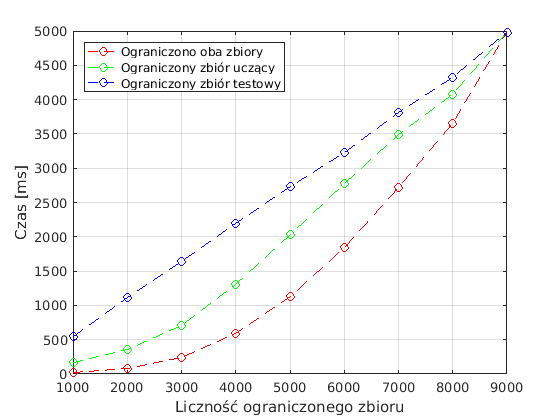
\includegraphics[width=11.5cm]{img/knn_compexity}
	\caption{Czasowa złożoność obliczeniowa algorytmu $KNN$.}
	\label{fig:knn_compexity}
\end{figure}
\begin{figure}[H]
	\centering
	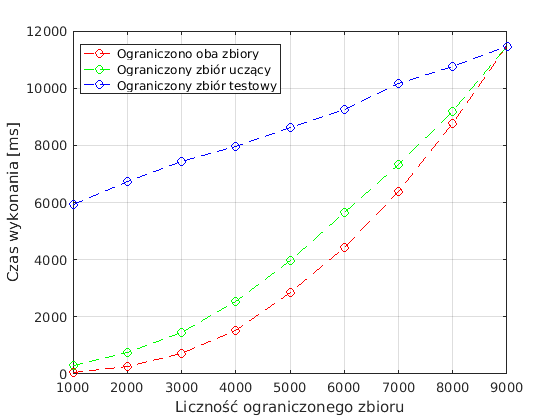
\includegraphics[width=11.5cm]{img/enn_complexity}
	\caption{Czasowa złożoność obliczeniowa algorytmu $KNN$.}
	\label{fig:enn_complexity}
\end{figure}

W trakcie eksperymentu manipulowano licznością zbioru testowego oraz uczącego. Badano działanie aplikacji dla zmiennej wielkości jednego zbioru przy liczności drugiego równej $9000$ oraz dla zbiorów o takiej samej wielkości w zakresie od $1000$ do $9000$ wektorów. W przypadku obu algorytmów zaobserwować można liniowy wzrost czasu wykonania przy manipulacji rozmiarem jednego zbioru oraz kwadratowy wzrost w przypadku zmiany wielkości obu zbiorów jednocześnie.

\subsection{Omówienie możliwości wykorzystania zrównoważonego zbioru uczącego?}

\subsection{Dokładne wyniki dla kilku fajnych plików}



